\documentclass[a4paper,11pt,fleqn,dvipsnames,oneside,openright]{memoir} 	% Openright aabner kapitler paa hoejresider (openany begge)

%%%% PACKAGES %%%%

% ¤¤ Oversaettelse og tegnsaetning ¤¤ %
\usepackage[utf8]{inputenc}					% Input-indkodning af tegnsaet (UTF8)
\usepackage[danish]{babel}					% Dokumentets sprog
\usepackage[T1]{fontenc}					% Output-indkodning af tegnsaet (T1)
\usepackage{ragged2e,anyfontsize}			% Justering af elementer
\usepackage{fixltx2e}						% Retter forskellige fejl i LaTeX-kernen
																			
% ¤¤ Figurer og tabeller (floats) ¤¤ %
\usepackage{graphicx} 						% Haandtering af eksterne billeder (JPG, PNG, EPS, PDF)

\usepackage{subfig}

%\usepackage{eso-pic}						% Tilfoej billedekommandoer paa hver side
%\usepackage{wrapfig}						% Indsaettelse af figurer omsvoebt af tekst. \begin{wrapfigure}{Placering}{Stoerrelse}
\usepackage[space]{grffile}					% Bør gøre det muligt at have mellemrum i filnavne.
\usepackage{multirow}                		% Fletning af raekker og kolonner (\multicolumn og \multirow)
\usepackage{multicol}         	        	% Muliggoer output i spalter
\usepackage{rotating}						% Rotation af tekst med \begin{sideways}...\end{sideways}
\usepackage{colortbl} 						% Farver i tabeller (fx \columncolor og \rowcolor)
\usepackage[usenames,dvipsnames]{xcolor}	% Definer farver med \definecolor. Se mere: http://en.wikibooks.org/wiki/LaTeX/Colors
%\usepackage{flafter}						% Soerger for at floats ikke optraeder i teksten foer deres reference
\let\newfloat\relax 						% Justering mellem float-pakken og memoir
\usepackage{float}							% Muliggoer eksakt placering af floats, f.eks. \begin{figure}[H]
\setlength{\heavyrulewidth}{0.15em}			% Sætter \toprule og \bottomrule til fast størrelse (0.08 er default)
%\setlength{\lightrulewidth}{0.05em}		% Sætter \midrule til fast størrelse (0.05 er default)
\usepackage{array}							% Bruges i forbindelse med \newcolumntype-command under egne commands
\usepackage{pdfpages}						% Bruges så der kan indsættes pdf, som sider (forside for eksempel)
\usepackage{wrapfig}
\usepackage[section]{placeins}				% Indsætter en border så billeder bliver placeret inden for den section de er indsat
\usepackage{lastpage}						% Anvendes til at se total antal sider

% ¤¤ Matematik mm. ¤¤
\usepackage{amsmath,amssymb,stmaryrd} 		% Avancerede matematik-udvidelser
\usepackage{mathtools}						% Andre matematik- og tegnudvidelser
\usepackage{textcomp}                 		% Symbol-udvidelser (f.eks. promille-tegn med \textperthousand )
\usepackage{rsphrase}						% Kemi-pakke til RS-saetninger, f.eks. \rsphrase{R1}
\usepackage[version=3]{mhchem} 				% Kemi-pakke til flot og let notation af formler, f.eks. \ce{Fe2O3}
\usepackage{siunitx}						% Flot og konsistent praesentation af tal og enheder med \si{enhed} og \SI{tal}{enhed}
\sisetup{locale=DE}							% Opsaetning af \SI (DE for komma som decimalseparator) 

% ¤¤ Referencer og kilder ¤¤ %
\usepackage[danish]{varioref}				% Muliggoer bl.a. krydshenvisninger med sidetal (\vref)
\usepackage{natbib}							% Udvidelse med naturvidenskabelige citationsmodeller
\usepackage{xr-hyper}							% Referencer til eksternt dokument med \externaldocument{<NAVN>}
\externaldocument[DokRap-]{../Dokumentationsrapport/Dokumentationsrapport}	% Muliggør eksterne referencer til dokumentationsrapporten
%\usepackage{glossaries}					% Terminologi- eller symbolliste (se mere i Daleifs Latex-bog)



% ¤¤ Misc. ¤¤ %
\usepackage{lipsum}							% Dummy text \lipsum[..]
\usepackage[shortlabels]{enumitem}			% Muliggoer enkelt konfiguration af lister
\usepackage{pdfpages}						% Goer det muligt at inkludere pdf-dokumenter med kommandoen \includepdf[pages={x-y}]{fil.pdf}	
\pdfoptionpdfminorversion=6					% Muliggoer inkludering af pdf dokumenter, af version 1.6 og hoejere
\pretolerance=2500 							% Justering af afstand mellem ord (hoejt tal, mindre orddeling og mere luft mellem ord)

% Kommentarer og rettelser med \fxnote. Med 'final' i stedet for 'draft' udloeser hver note en error i den faerdige rapport.
\usepackage[footnote,draft,danish,silent,nomargin]{fixme}	

%lists
\usepackage{listings}	


%%%% CUSTOM SETTINGS %%%%

% ¤¤ Marginer ¤¤ %
\setlrmarginsandblock{3.5cm}{2.5cm}{*}		% \setlrmarginsandblock{Indbinding}{Kant}{Ratio}
\setulmarginsandblock{2.5cm}{3.0cm}{*}		% \setulmarginsandblock{Top}{Bund}{Ratio}
\checkandfixthelayout 						% Oversaetter vaerdier til brug for andre pakker

%	¤¤ Afsnitsformatering ¤¤ %
\setlength{\parindent}{0mm}           		% Stoerrelse af indryk
\setlength{\parskip}{3mm}          			% Afstand mellem afsnit ved brug af double Enter
\linespread{1,1}							% Linie afstand
\newcommand{\tab}{\hspace*{2em}}			% ved \tab{} indrykkes det i klammerne ind
\usepackage{titlesec}							%Muliiggøre ændring af sections i alle lag
\titleformat*{\section}{\LARGE\bfseries\color{NavyBlue}}		%section = størst
\titleformat*{\subsection}{\Large\bfseries\color{RoyalBlue}}		%sub og subsub har samme størrelse
\titleformat*{\subsubsection}{\Large\bfseries}
\titleformat*{\paragraph}{\large\bfseries}		%Benyttes umiddelbart ikke
\titleformat*{\subparagraph}{\large\bfseries}	%Benyttes umiddelbart ikke

% ¤¤ Litteraturlisten ¤¤ %
\bibpunct[,]{[}{]}{;}{a}{,}{,} 				% Definerer de 6 parametre ved Harvard henvisning (bl.a. parantestype og seperatortegn)
\bibliographystyle{bibtex/harvard}			% Udseende af litteraturlisten.

% ¤¤ Indholdsfortegnelse ¤¤ %
\setsecnumdepth{subsubsection}		 		% Dybden af nummerede overkrifter (part/chapter/section/subsection)
\maxsecnumdepth{subsection}					% Dokumentklassens graense for nummereringsdybde
\settocdepth{subsubsection} 				% Dybden af indholdsfortegnelsen

% ¤¤ Lister ¤¤ %
\setlist{
  topsep=-5pt,								% Vertikal afstand mellem tekst og listen	Default: 0
  itemsep=-1ex,								% Vertikal afstand mellem items
} 

% ¤¤ Visuelle referencer ¤¤ %
\usepackage[colorlinks]{hyperref}			% Danner klikbare referencer (hyperlinks) i dokumentet.
\hypersetup{colorlinks = true,				% Opsaetning af farvede hyperlinks (interne links, citeringer og URL)
    linkcolor = black,
    citecolor = black,
    urlcolor = black
}

% ¤¤ Opsaetning af figur- og tabeltekst ¤¤ %
\usepackage{caption}
\captionnamefont{\small\bfseries\itshape}	% Opsaetning af tekstdelen ('Figur' eller 'Tabel')
\captiontitlefont{\small}					% Opsaetning af nummerering
\captiondelim{. }							% Seperator mellem nummerering og figurtekst
\hangcaption								% Venstrejusterer flere-liniers figurtekst under hinanden
\captionsetup{width=\linewidth,labelfont={bf,it}}
\setlength{\abovecaptionskip}{5pt}			% Afstand over figurteksten
\setlength{\belowcaptionskip}{-12pt}		% Afstand under figurteksten
		
% ¤¤ Navngivning ¤¤ %
\addto\captionsdanish{
	\renewcommand\appendixname{Appendiks}
	\renewcommand\contentsname{Indholdsfortegnelse}	
	\renewcommand\appendixpagename{Appendiks}
	\renewcommand\appendixtocname{Appendiks}
	\renewcommand\cftchaptername{\chaptername~}				% Skriver "Kapitel" foran kapitlerne i indholdsfortegnelsen
	\renewcommand\cftappendixname{\appendixname~}			% Skriver "Appendiks" foran appendiks i indholdsfortegnelsen
}

% ¤¤ Kapiteludssende ¤¤ %
\definecolor{chapnumcolor}{RGB}{23,54,93}		% Definerer en farve til brug til kapiteludseende
\definecolor{chapfontcolor}{RGB}{29,69,118}
\newif\ifchapternonum

\makechapterstyle{jenor}{					% Definerer kapiteludseende frem til ...
  \renewcommand\beforechapskip{0pt}
  \renewcommand\printchaptername{}
  \renewcommand\printchapternum{}
  \renewcommand\printchapternonum{\chapternonumtrue}
  \renewcommand\chaptitlefont{\fontfamily{pbk}\fontseries{db}\fontshape{n}\fontsize{25}{35}\selectfont\raggedleft\color{chapfontcolor}}
  \renewcommand\chapnumfont{\fontfamily{pbk}\fontseries{m}\fontshape{n}\fontsize{1in}{0in}\selectfont\color{chapnumcolor}}
  \renewcommand\printchaptertitle[1]{%
    \noindent
    \ifchapternonum
    \begin{tabularx}{\textwidth}{X}
    {\let\\\newline\chaptitlefont ##1\par} 
    \end{tabularx}
    \par\vskip-2.5mm\hrule
    \else
    \begin{tabularx}{\textwidth}{Xl}
    {\parbox[b]{\linewidth}{\chaptitlefont ##1}} & \raisebox{-15pt}{\chapnumfont \thechapter}
    \end{tabularx}
    \par\vskip2mm\hrule
    \fi
  }
}											% ... her

\chapterstyle{jenor}						% Valg af kapiteludseende - Google 'memoir chapter styles' for alternativer

% ¤¤ Sidehoved ¤¤ %

\makepagestyle{AAU}							% Definerer sidehoved og sidefod udseende frem til ...
\makepsmarks{AAU}{%
	\createmark{chapter}{left}{shownumber}{}{. \ }
	\createmark{section}{right}{shownumber}{}{. \ }
	\createplainmark{toc}{both}{\contentsname}
	\createplainmark{lof}{both}{\listfigurename}
	\createplainmark{lot}{both}{\listtablename}
	\createplainmark{bib}{both}{\bibname}
	\createplainmark{index}{both}{\indexname}
	\createplainmark{glossary}{both}{\glossaryname}
}
\nouppercaseheads											% Ingen Caps oenskes

\makeevenhead{AAU}{Test}{}{\leftmark}					% Definerer lige siders sidehoved (\makeevenhead{Navn}{Venstre}{Center}{Hoejre})
\makeoddhead{AAU}{\rightmark}{}{Ingeniørhøjskolen, Aarhus Universitet}		% Definerer ulige siders sidehoved (\makeoddhead{Navn}{Venstre}{Center}{Hoejre})
\makeevenfoot{AAU}{\thepage}{}{}							% Definerer lige siders sidefod (\makeevenfoot{Navn}{Venstre}{Center}{Hoejre})
\makeoddfoot{AAU}{}{}{\thepage}								% Definerer ulige siders sidefod (\makeoddfoot{Navn}{Venstre}{Center}{Hoejre})
\makeheadrule{AAU}{\textwidth}{0.5pt}						% Tilfoejer en streg under sidehovedets indhold
\makefootrule{AAU}{\textwidth}{0.5pt}{1mm}					% Tilfoejer en streg under sidefodens indhold

\copypagestyle{AAUchap}{AAU}								% Sidehoved for kapitelsider defineres som standardsider, men med blank sidehoved
\makeoddhead{AAUchap}{}{}{}
\makeevenhead{AAUchap}{}{}{}
\makeheadrule{AAUchap}{\textwidth}{0pt}
\aliaspagestyle{chapter}{AAUchap}							% Den ny style vaelges til at gaelde for chapters
															% ... her
															
\pagestyle{AAU}												% Valg af sidehoved og sidefod



% Opsætning af source code import
% \lstinputlisting{sti../navn.endelse}
\lstset{
  language=C,                		% choose the language of the code
  numbers=left,                   	% where to put the line-numbers
  stepnumber=1,                   	% the step between two line-numbers.        
  numbersep=5pt,                  	% how far the line-numbers are from the code
  backgroundcolor=\color{white},  	% choose the background color. You must add \usepackage{color}
  showspaces=false,               	% show spaces adding particular underscores
  showstringspaces=false,         	% underline spaces within strings
  showtabs=false,                 	% show tabs within strings adding particular underscores
  tabsize=2,                      	% sets default tabsize to 2 spaces
  captionpos=b,                   	% sets the caption-position to bottom
  breaklines=true,                	% sets automatic line breaking
  breakatwhitespace=true,         	% sets if automatic breaks should only happen at whitespace
  title=\lstname,                 	% show the filename of files included with \lstinputlisting;
  emph={ uint8, uint16, void }, emphstyle={\color{blue}}	% tilføj variabel hvis de skal markeres blå
}






%%%% CUSTOM COMMANDS %%%%

% ¤¤ Billede hack ¤¤ %
\newcommand{\figur}[4]{
		\begin{figure}[H] \centering
			\includegraphics[width=#1\textwidth]{Billeder/#2}
			\caption{#3}\label{#4}
		\end{figure} 
}


% ¤¤ Venstre orienterer al tekst i p{Ycm} ¤¤ %
\newcolumntype{x}[1]{%
>{\raggedright\hspace{0pt}}p{#1}}

% ¤¤ Newline til x{} ¤¤ %
% \\ virker åbenbart ikke når man selv laver en columntype... :(
\newcommand{\tn}{\tabularnewline}

% ¤¤ Newline til x{} ¤¤ %
% \\ virker åbenbart ikke når man selv laver en columntype... :(
\newcommand{\tnhl}{\tabularnewline\hline}



% ¤¤ Nyt environment til indsættelse af A3-størrelse figurer
\newenvironment{A3Figure}
{
	\cleardoublepage
	\pageaiii
	\setlength{\pdfpagewidth}{\paperheight} % Change the pdf page to A3 height
	\setlength{\pdfpageheight}{\paperwidth} % Change the pdf height to A3 width
	\setlength{\textwidth}{\paperheight - \the\spinemargin-\the\foremargin} % Change the textwidth
}
{
	\cleardoublepage	
}

% funktions beskrivelse void argument%
\newcommand{\funcDescrip}[2]{
\textbf{{\color{blue} #1} #2({\color{blue} void})} \\
}

% funktions beskrivelse 1 argument%
\newcommand{\funcDescripOne}[4]{
\textbf{{\color{blue} #1} #2({\color{blue} #3} #4)} \\
}

% funktions beskrivelse 2 argument%
\newcommand{\funcDescripTwo}[6]{
\textbf{{\color{blue} #1} #2({\color{blue} #3} #4, {\color{blue} #5} #6)} \\
}

% opsætning af funktions tabel %
\newcommand{\funcTabel}[4]{
\begin{tabular}{p{0.2cm}p{3cm}p{11cm}} \hline
	&	\textbf{Description:} 		& 	#1	\\
	&	\textbf{Parameters:} 		& 	#2	\\
	&	\textbf{Return Value:}		& 	#3	\\
	&	\textbf{Side Effects:}		&	#4	\\
\end{tabular}
}


% ¤¤ Units i math-environments ¤¤ %
\newcommand{\mathUnit}[2]{\mathrm{\si{#1}{#2}}}







% ¤¤ Pæn opsætning af titelblad-dele ¤¤ %
% ¤¤ Husk at ændre dato i senere projekter ¤¤ %
\newcommand{\titelblad}[2]{
\begin{tabular}[ht]{x{7cm}x{7cm}}
\textbf{Navn: } #1		&\textbf{Studienummer: } #2	\tn
\textbf{Dato} 2013-05-31	\tn
\multicolumn{2}{l}{\textbf{Underskrift: }\line(1,0){340}}
\end{tabular}
}


% ¤¤ Specielle tegn ¤¤ %
\newcommand{\grader}{^{\circ}\text{C}}   % Grader C, virker kun i math-environments
\newcommand{\gr}{^{\circ}}
\newcommand{\g}{\cdot}		% Gange i math-environments
\newcommand{\grC}{$^{\circ}\mathrm{C}$}		% Grader C, uden for math-environments

%%%% ORDDELING %%%%

\hyphenation{}

%%%Indsat af Søren%%%
\usepackage{listings}
\usepackage{color}
 
\definecolor{dkgreen}{rgb}{0,0.6,0}
\definecolor{gray}{rgb}{0.5,0.5,0.5}
\definecolor{mauve}{rgb}{0.58,0,0.82}
 
\lstset{ %
  language=Octave,                % the language of the code
  basicstyle=\footnotesize,           % the size of the fonts that are used for the code
  numbers=left,                   % where to put the line-numbers
  numberstyle=\tiny\color{gray},  % the style that is used for the line-numbers
  stepnumber=2,                   % the step between two line-numbers. If it's 1, each line 
                                  % will be numbered
  numbersep=5pt,                  % how far the line-numbers are from the code
  backgroundcolor=\color{white},      % choose the background color. You must add \usepackage{color}
  showspaces=false,               % show spaces adding particular underscores
  showstringspaces=false,         % underline spaces within strings
  showtabs=false,                 % show tabs within strings adding particular underscores
  frame=single,                   % adds a frame around the code
  rulecolor=\color{black},        % if not set, the frame-color may be changed on line-breaks within not-black text (e.g. comments (green here))
  tabsize=2,                      % sets default tabsize to 2 spaces
  captionpos=b,                   % sets the caption-position to bottom
  breaklines=true,                % sets automatic line breaking
  breakatwhitespace=false,        % sets if automatic breaks should only happen at whitespace
  title=\lstname,                   % show the filename of files included with \lstinputlisting;
                                  % also try caption instead of title
  keywordstyle=\color{blue},          % keyword style
  commentstyle=\color{dkgreen},       % comment style
  stringstyle=\color{mauve},         % string literal style
  escapeinside={\%*}{*)},            % if you want to add LaTeX within your code
  morekeywords={*,...},              % if you want to add more keywords to the set
  deletekeywords={...}              % if you want to delete keywords from the given language
}											% Preamble 
\raggedbottom													% LaTeX "straekker" ikke teksten

%\includeonly{file1,file2}										% Inkluder kun specifikke filer 

\begin{document}												% Starter
\frontmatter													% Forindhold - nummereres med romertal
\thispagestyle{empty}
\begin{flushright}
\vspace{3cm}

\phantom{hul}

\phantom{hul}

\phantom{hul}

\textsl{\Huge Skeleton Project} \\ \vspace{1cm}

\rule{13cm}{3mm} \\ \vspace{1.5cm}
\vspace{1cm}


\includegraphics[width=0.4\textwidth]{4.Construction/pictures/skeleton-cover.jpg}

\vspace{2cm} 
\textsc{\Large Skeleton Project V1 \\
Group of project \\
Faculty\\
Delivery date\\}
\end{flushright}

 %%%%%% Resumé %%%%%%
\chapter{Resumé og Abstract}
\label{chap:resume}


\section*{Abstract}


\section*{Resumé}

Formålet med dette bachelorprojekt er at udvikle en overvågningsdrone der nemt og omkostningsfrit kan overvåge et område. Dronen udvikles for at skabe et alternativ til dyr og ressourcekrævende overvågning udført af mennesker.
Projektet er designet og udviklet på Ingeniørhøjskolen Aarhus Universitet.

I projektet omdannes en fjernstyret quadrocopter til en drone, som skal bruges til overvågning. Ud fra brugers anvisninger skal drone autonomt kunne flyve til GPS positioner og tage overvågningsbilleder.  

Den udviklede drone består af en Aeroquad ARF quadrocopter med påmonteret GPS, højdemåler og mobilt kommunikationsmodul. Systemets bruger indstille droneflyvning samt monitorerer data fra tidligere flyvninger via en webapplikation.  

I projektforløbet lykkedes det at implementere en fuldt fungerende server, samt kommunikationslink og udveksling af data mellem server og drone. Desuden blev opsamling af data fra GPS, kompas og højdemåler fuldt ud implementeret. Det lykkedes endvidere at implementere hovedparten af webapplikationen og dronens autonome flyvning.







%%%% Indholdsfortegnelse (TOC) %%%%
\tableofcontents*												%Indholdsfortegnelsen (kaldet ToC) 

\mainmatter														% Hovedindhold - nummereres fra side 1




\chapter{Systemarkitektur}

\section{Revisionshistorik}
\begin{table}[H]
	\centering
		\begin{tabular}{|p{2 cm}|p{2 cm}|p{3 cm}|p{6 cm}|} 
		\hline
			\textbf{Rev. Nr} & \textbf{Dato}		& \textbf{Initialer} 	& \textbf{Ændring} \\ \hline
			1.0 	& & &  \\ \hline
			1.1 	& & &	\\ \hline
		\end{tabular}
	\caption{Revisionshistorik}
	%\label{tab:TC1}
\end{table}

\vspace{1.5cm}

\section{Ordforklaring}
\begin{table}[H]
	\centering
		\begin{tabular}{|p{2.5cm}|p{4.5 cm}|p{6.5 cm}|} 
		\hline
			\textbf{Forkortelse} & \textbf{Betydning} & \textbf{Forklaring} \\ \hline
			 &  &  \\ \hline
			 &  & \\ \hline
		\end{tabular}
	\caption{Ordforklaring}
	%\label{tab:TC1}
\end{table}

\vspace{2cm}

\section{Indledning}
Dette kapitel beskriver hvilke enheder systemet består af samt grænseflader mellem
enhederne. Til at beskrive hardware og tilhørende grænseflader benyttes SysML diagrammer, mens software og tilhørende grænseflader beskrives med UML diagrammer.

\chapter{Forord}

Dette projekt blev tilbudt som et bachelorprojekt af Ingeniørhøjskolen Aarhus Universitet. Grundet tidens stigende fokus på droner ønskede Ingeniørhøjskolen det undersøgt hvorvidt det var muligt at udvikle en drone.

Der var i udgangspunkt ingen begrænsninger for hvad bachelorprojektet kunne eller skulle indeholde. Derfor har gruppen på egen hånd opsat krav, designet og udformet bachelorprojektet \textit{Autonom overvågningsdrone}.
 
Projekt, projektrapport og tilhørende dokumentationen er udarbejdet af projektgruppe 14123, bestående af 3 ingeniørstuderende. Gruppen er blevet bevilliget økonomisk støtte til indkøb af drone, sensorer og andet hardware. Ydermere har gruppen fået vejledning og rådgivning af en vejleder tilknyttet fra Ingeniørhøjskolen Aarhus Universitet.  \\


\subsection*{\textit{Referencer} \vspace{-0.3cm}}
Betegnelsen [x] hentyder til en reference, som står i referencelisten sidst i rapporten. 
%%%%%% Indledning %%%%%%
\chapter{Indledning}
\label{chap:indledning}

I den moderne verden findes der mange forskellige former for overvågning, og overvågning foregår overalt. Primært bruges overvågning til at skabe tryghed og forebygge mod kriminalitet, hvilket de fleste mennesker er positivt stemt overfor. Men pga. en stigning i brugen af overvågning, bruges der gradvist flere og flere ressourcer på området. 
I projektet undersøges det, hvorvidt det er muligt at udvikle en autonom overvågningsdrone. Det er gruppens mål at udvikle en drone der ud fra administrators anvisninger kan overvåge og tage billeder af et defineret område. Dronen udvikles for at mindske mængden af menneskelige ressourcer der bruges på overvågning.

Formålet med projektet er at konstruere en drone, som autonomt kan overvåge et givet område. Dronen gøres i stand til at kommunikere med en server, samt orientere sig om egen GPS position, flyvehøjde og flyveretning. Gennem kommunikation med server henter dronen flyveopsætning og flyver på egen hånd ud og overvåger et defineret område.
Projektet er planlagt, designet og konstrueret hen over en periode på 4 måneder.

Projektrapporten er sat op efter en standard, hvor systemet indledningsvis beskrives på et abstrakt niveau. Herefter beskrives krav til produktet, og der gåes mere analytisk og teknisk til værks. Rapporten afsluttes af med resultater, diskussion af resultater samt en konklusion.




\chapter{Systembeskrivelse}
\vspace{-1cm}
På Ingeniørhøjskolen Aarhus Universitet forefindes en AeroQuad ARF Quadrocopter. 
Målet med projektet er at omdanne quadrocopteren til en autonom overvågningsdrone.

Dronen skal ud fra brugers anvisninger overvåge og tage billeder af et defineret område. 
Dronen tilgås via en webapplikation der fungerer som en grafisk brugerflade mellem bruger og systemet.  Via webapplikationen kan bruger oprette flyveopsætninger til drone samt se billeder og flyverute fra tidligere flyvninger.  
Når der laves ny flyveopsætning vælger bruger en række GPS positioner som dronen skal flyve til, flyvehøjde og hvorvidt der skal tages billeder ved de valgte GPS positioner. Når bruger har lavet en ny flyveopsætning, stilles flyveopsætningen tilgængelig for dronen på server.  

Da dronen skal flyve autonomt, er det vigtigt den kan orientere sig på egen hånd. Derfor er dronen udstyret med GPS, afstands sensorer og kompas.
Til enhver tid, skal kommunikation mellem drone og server foregå via mobilt netværk. Der gøres hovedsageligt brug af 3G netværket, men i områder med dårlig forbindelse vil der blive gjort brug af 2G som fall-back netværk. 

\vspace{-0.5cm}

\section*{Systemskitse}
\vspace{-0.5cm}
Bruger benytter en computer til at tilgå webapplikation og lave en ny flyveopsætning. Når bruger har lavet en ny flyveopsætning, overføres flyveopsætningen via internettet til server, hvor den gøres tilgængelig for dronen.
 
Via det mobile 3G netværk kommunikerer drone med server. 
Inden flyvning påbegyndes henter drone flyveopsætning fra server og under flyvning sender dronen information om nuværende GPS position og overfører billeder til server. 
Under flyvning kontrollerer drone løbende egen GPS position via kommunikation med GPS satellitter. Dette gør den for at opdatere egen position og for efterfølgende at kunne beregne den korrekte flyveorientering. 



\vspace{-5pt}
%Systemskitse
\begin{figure}[H]
\centering
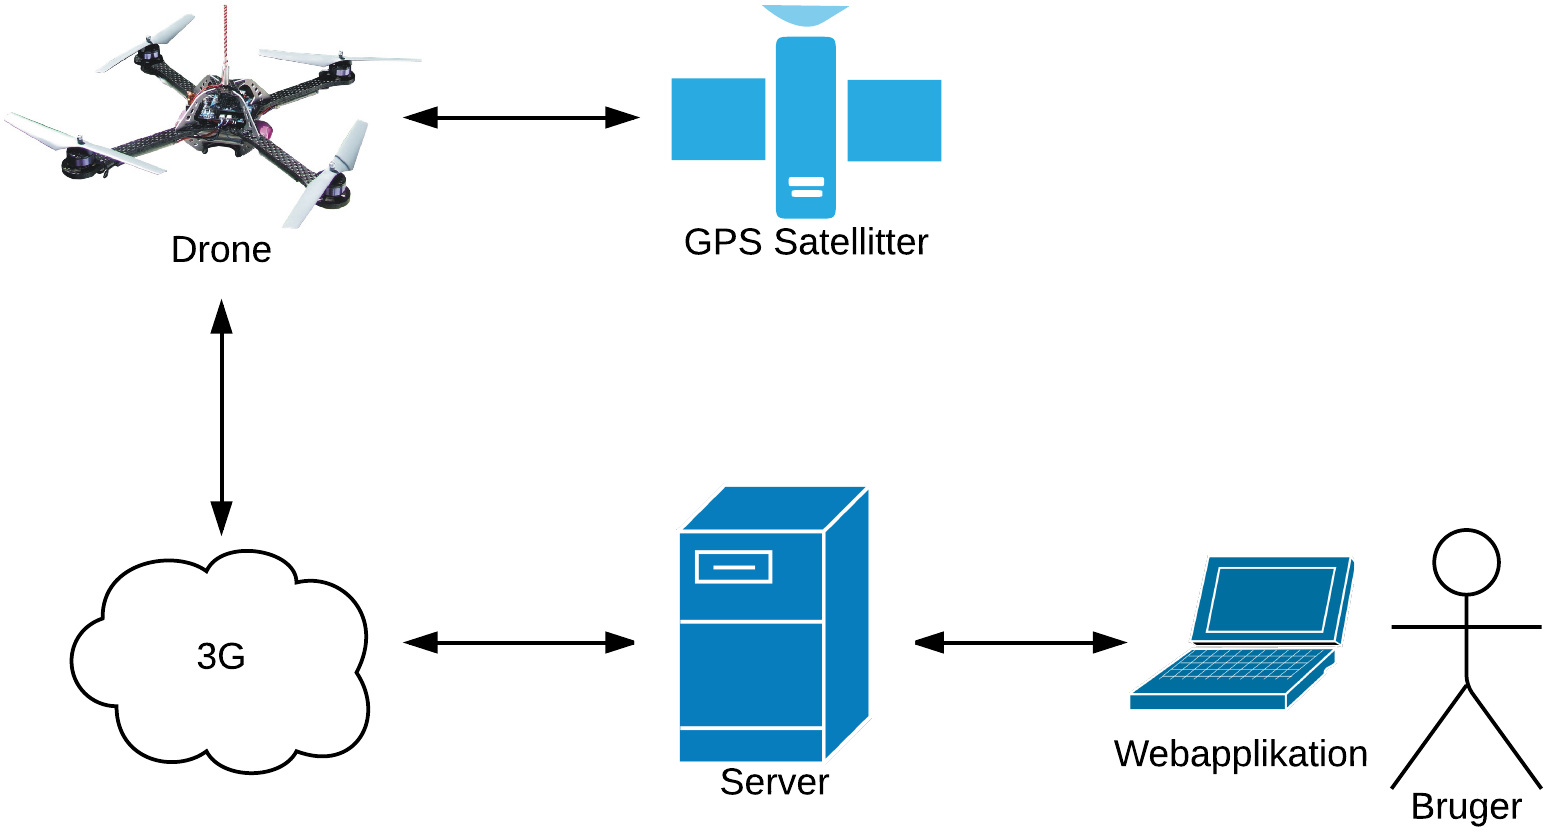
\includegraphics[width=1\textwidth]{Billeder/Projektbeskrivelse.png}
\vspace{-.5cm}
\caption{Systemskitse}
\label{fig:Systemskitse}
\end{figure}
%%%%%% Krav %%%%%%
\chapter{Krav}
\vspace{-0.5cm}
I dette afsnit beskrives kravene til projektet [1]. Indledningsvis præsenteres funktionelle krav  ved brug af use cases. På figur \ref{fig:useCaseDiagram} vises et use diagram, der viser aktører og use cases tilhørende systemet. Efter use case diagrammet følger en kort beskrivelse af de seks use cases og deres funktion. Afsnittet afsluttets med ikke-funktionelle krav, der er både er krav til systemet som helhed og til systemets blokke.
\vspace{-0.3cm}

\section{Funktionelle krav}
\vspace{-0.2cm}
Til systemet er der identificeret de 2 aktører: Bruger \& GPS-satellitter. Bruger er primær aktør der ønsker at initialisere og styre systemet. Bruger er ansvarlig for at oprette flyveopsætninger på webapplikationen og tilslutte batteri til dronen.
GPS-satellitter er sekundær aktør, der gør det muligt for dronen at finde egen position. 
På figur \ref{fig:useCaseDiagram} vises et use case diagram, der viser systemets aktørerne og i hvilke use cases aktørerne optræder. 
\begin{figure}[H]
	\centering
	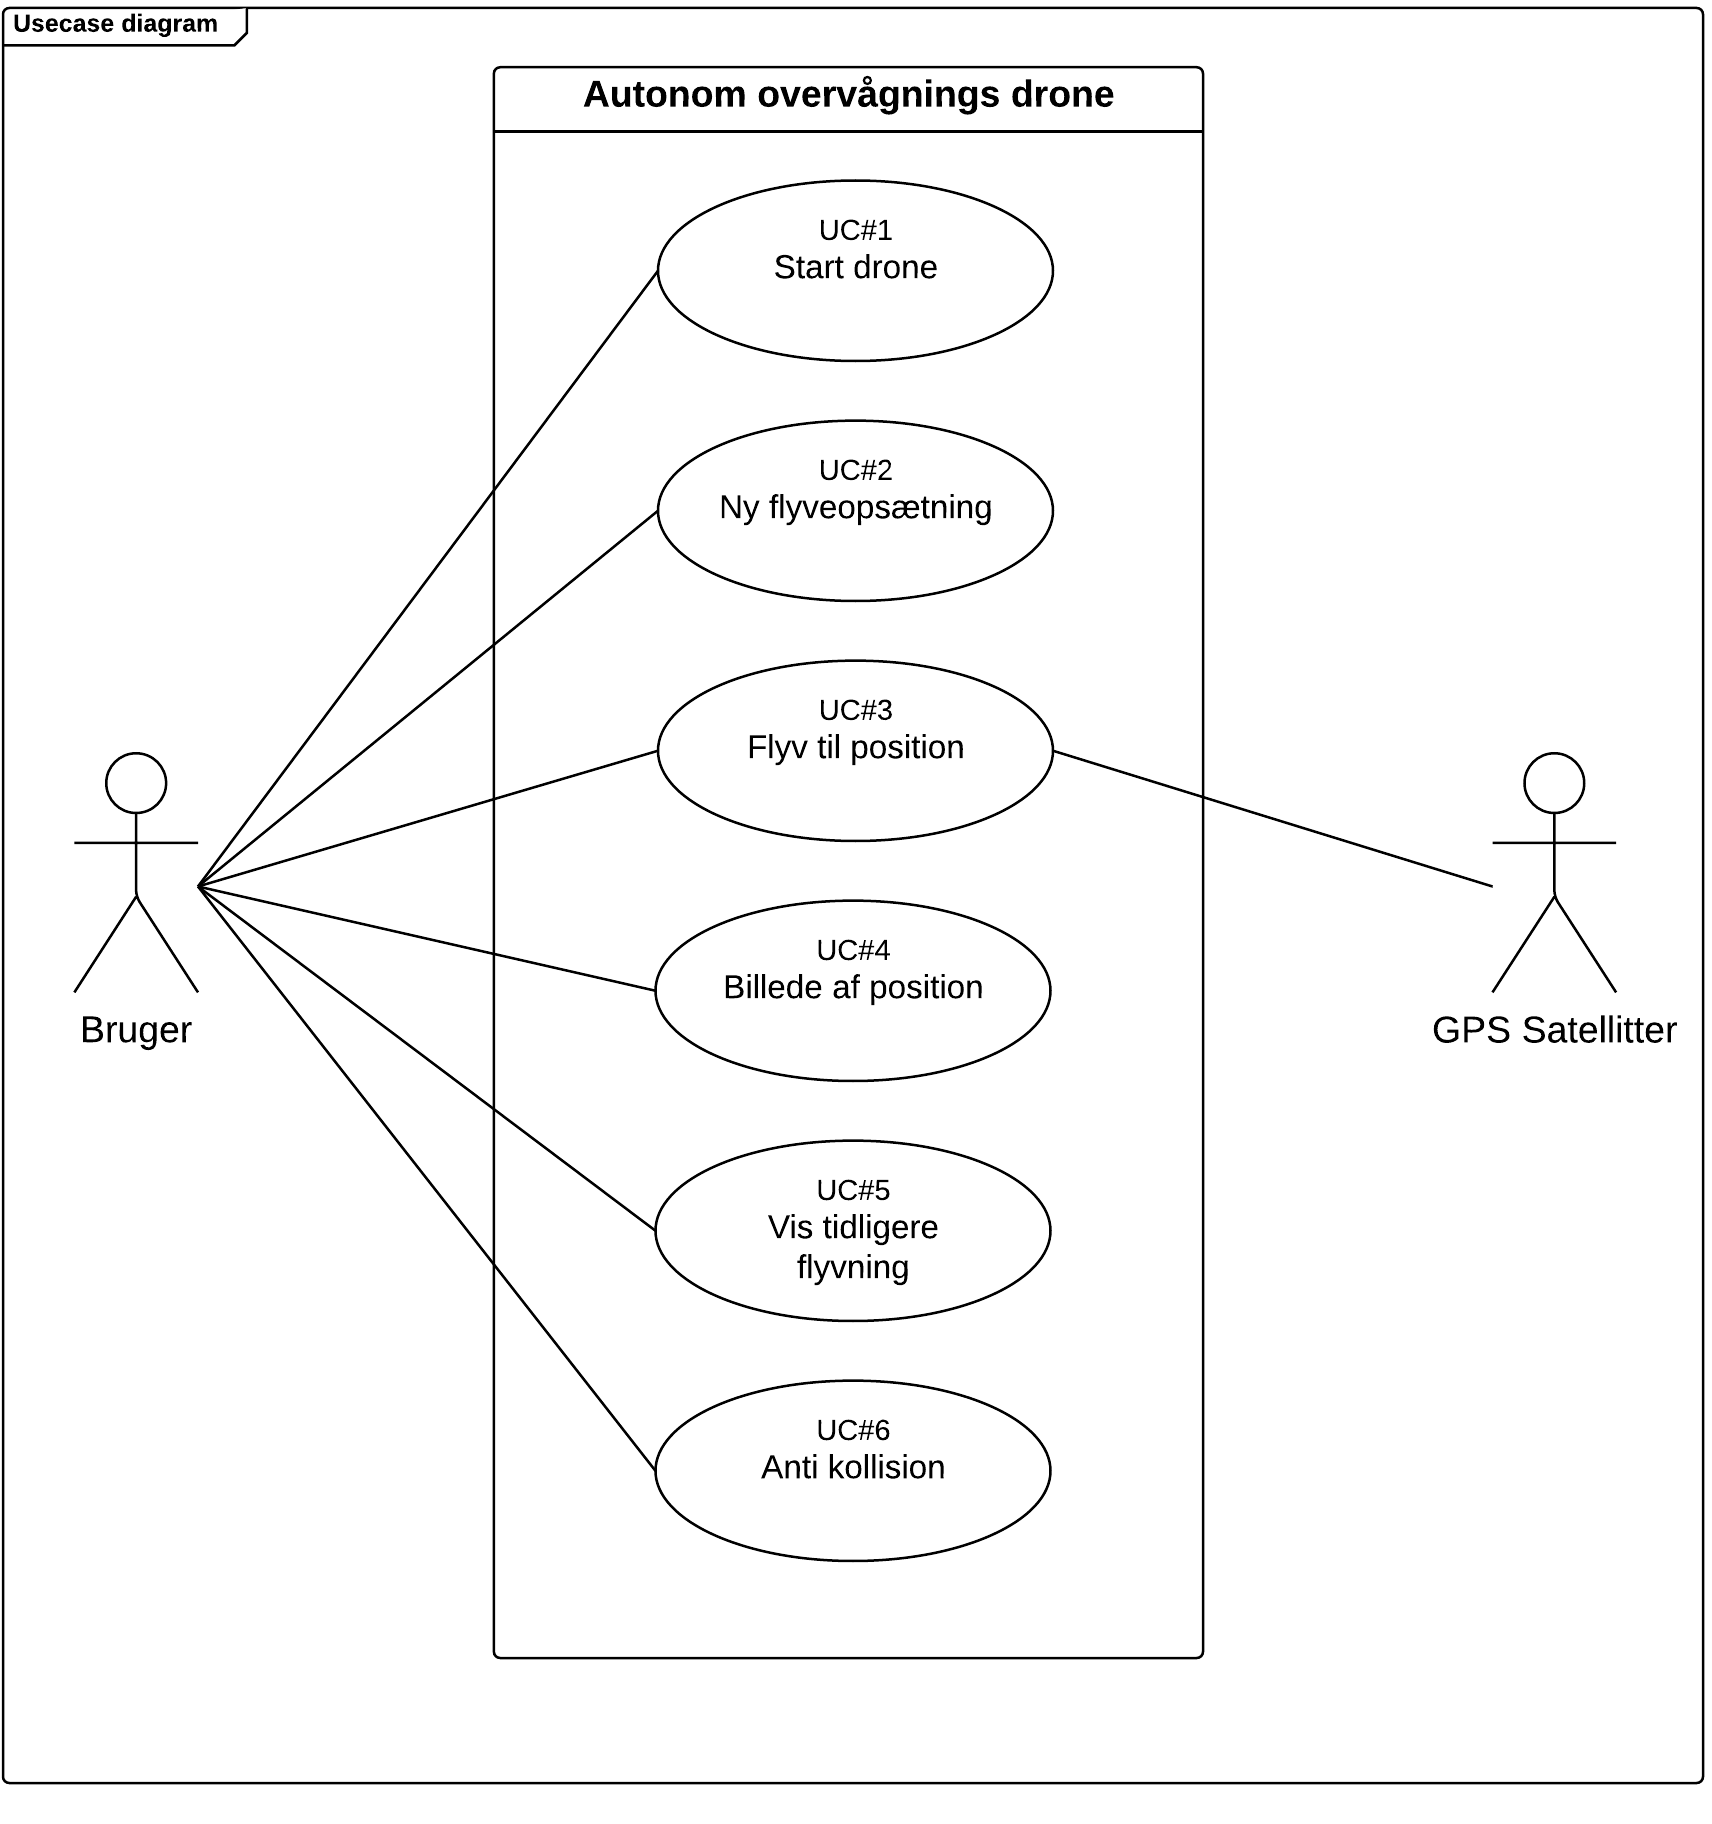
\includegraphics[width=0.75\textwidth]{Billeder/Krav/Use_case_diagram}
	\vspace{-0.3cm}	
	\caption{Use case diagram}
	\label{fig:useCaseDiagram}
\end{figure}

\newpage

I projektets kravspecifikation er alle use cases beskrevet som fully dressed use cases. I fully dressed use cases beskrives hvordan hovedforløb ser ud i en given use case, hvis den succesfuldt gennemføres. Desuden beskrives startbetingelse, aktører og tilføjelser.

Nedenfor beskrives hovedforløb og funktion af de seks use cases:\\

\textbf{Use case 1: Start drone} \\
Bruger tilslutter batteri til drone og dronen initialiseres. Drone sender information om nuværende position til server.\\

\textbf{Use case 2: Ny flyveopsætning} \\
Bruger logger på webapplikation og opretter en ny flyveopsætning. Flyveopsætningen sættes tilgængelig for drone på server.\\

\textbf{Use case 3: Flyv til position}\\
Drone henter flyveopsætning fra server og påbegynder flyvning. Under flyvning tilpasser drone  løbende flyvehøjde og flyveorientering og fortsætter flyvning mod ønsket position. \\

\textbf{Use case 4: Billede af position} \\
Når drone er ankommet til ønsket GPS position tages et billede. Hvis billedet accepteres, flyver dronen videre mod næste GPS koordinat eller til udgangsposition. \\

\textbf{Use case 5: Vis tidligere flyvninger} \\
Bruger tilgår webapplikation for at se flyveruter og billeder tidligere flyvninger.\\

\textbf{Use case 6: Antikollision} \\
Drones antikollisions sensorer bruges til at detekterer forhindringer. I tilfælde af forhindringer ændre drone enten flyveretning eller flyvehøjde for at undgå kollision. \\



\section{Ikke-funktionelle krav}

De ikke-funktionelle krav opstilles ud fra systemspecifikationerne og er krav som ikke kan defineres i use cases. Disse krav har ingen indvirkning på systemets endelig funktion, kun systemspecifikationer.  

De ikke-funktionelle krav opstilles i fem grupper. Nogle krav er generelle krav til systemet, mens andre krav mere specifikt omhandler drone, server og webapplikation eller dataopsamling. 
De ikke-funktionelle krav bruges til at sikre system performance, eksempelvis stilles krav til de hardwaremoduler og sensorer der er monteret på dronen. 

\section{Projektafgrænsning}

Det er blevet vedtaget at implementere systemet som vist på figur ???????.
Der blev fra dag et af besluttet at afgrænse systemets omfang, således at der kunne sættes et realistisk mål i forhold til projekts omfang. \\
Et af afgrænsningerne var videokameraet. Det var tiltænkt at dronen skulle have et videokamera fast monteret, som skulle bruges til at live streame, i samme stil som hvis et stationært overvågningskamera blev anvendt.
Derudover blev der besluttet at nøjes med at bruge lavere kvalitets billeder, for  at gøre upload tiden mindre og derved fokusere på flyvningen.

I kravspecifikationen beskrives det at ethvert device med internet adgang kan benytte webapplikationen. Afhængigt af hvilket device der benytter webapplikationen, kræves en ny opsætning. Derfor er det besluttet kun at designe og implementere webapplikationen til en computer.

Flyvehøjde - bevidst valg af teknologi til højdemåling
Flyvehøjden til tests er bevidst valgt til at være under 5m. Dette skyldes valg af sensorer, da den valgte teknologi der anvendes har en maksimal rækkevidde på 5m. Derudover er højden valgt for at have mere kontrol over dronen under flyvning. 

Projektet blev opdelt i iterationer. Der blev valgt 4 iterationer, hvor den første iteration har den største prioritet, mens den sidste iteration prioriteres mindre højt. Dette medfører at man sikrer at de vigtigste dele af systemet implementeres først. Disse iterationer er beskrevet i projektets dokumentation[x].


\section{Udviklingsproces}
Projektforløbet er gennemført over en periode på 4 måneder, hvor der er blevet gjort brug af forskellige arbejdsmetoder og værktøjer. I dette afsnit beskrives hvorledes projektet er gennemført, hvilke metoder der er anvendt samt hvilke udviklingsværktøjer der er benyttet.

\subsection{Gennemførelse}
Under hele projektforløbet har alle gruppens medlemmer arbejdet tæt sammen. Specielt i starten af projektet hvor foranalyse, krav og indledende systemarkitektur blev udarbejdet, arbejdede gruppens medlemmer i tæt fællesskab. 
Da projektet bevægede sig over i detaljeret design og implementering, blev der gjort brug af iterativ udvikling, og gruppens medlemmer blev ansvarlige for forskellige dele. Foruden iterativ udvikling blev der også gjort brug af agil udvikling.


\subsubsection*{Iterativ udvikling}
Stort set alle udviklingsprojekter forløber via vandfaldsmodel eller iterativ udvikling. 
Hvis vandfaldsmodellen benyttes gennemløber projektet en række faser, der hver for sig afsluttes, inden næste fase påbegyndes. Opbygning af vandfaldsmodellen kunne eksempelvis være: Krav, analyse, design, implementering og test.
I et iterativt projektforløb gennemløber projektet i stedet en række iterationer, der hver for sig kan ses som miniudgaver af vandfaldsmodellen. Iterationer, der ligger tidligt i et projektforløb, vil ofte omhandle grundfunktionalitet, mens iterationer senere i projektforløbet bruges til at tilføje funktionalitet til systemet. 

\newpage 

Da krav til systemets funktionalitet var beskrevet med use cases, var det oplagt at opdele detaljeret design og implementering  i iterationer. Derfor blev detaljeret design og implementering opdelt i de fire iterationer, som beskrives nedenfor.  

\textbf{Iteration 1}\\
I første iteration er fokus på systemets mest grundlæggende funktionalitet. 
Drone gøres i stand til at oprette forbindelse til server via 3G/GPS-modulet.
Desuden tilsluttes batteri, ESC'er, motorer og ultralydssensor til drone. 
Målet med iterationen er at kunne gennemføre use case 1. 

\textbf{Iteration 2}\\
I iteration 2 er hovedformålet at få kommunikation mellem server og drone til at fungere. Bruger skal kunne oprette nye flyveopsætninger og gøre dem tilgængelige på server for dronen. Ydermere skal drone kunne finde egen GPS position, flyvehøjde og orientering. Ud fra viden om egen position, flyvehøjde og orientering skulle dronen kunne flyve til lokationer som er forudbestemt af bruger. Efter denne iteration skal use case 2 og 3 kunne gennemføres.

\textbf{Iteration 3}\\
I iteration 3 er hovedformålet at tilføje billede håndtering. Der monteres kamera på drone, så der kan tages billeder under flyvning. Billeder taget under flyvning sendes via mobilnet fra drone til server og gøres tilgængelige for bruger. Målet med iteration 3 er at kunne gennemføre use case 4 og 5.

\textbf{Iteration 4}\\
I iteration 4 er hovedformålet at udvikle antikollision til dronen. Inden tilføjelsen af antikollision kunne dronen udelukkende flyve i lukkede områder uden forhindringer. Tilføjelsen af antikollision skal muliggøre flyvning i normale områder med forhindringer. Efter denne iteration skal alle use cases kunne gennemføres.


\subsubsection*{Agile arbejdsmetoder}
Agil systemudvikling har fokus på løbende at levere værdi til kunden gennem en fleksibel og omskiftelig udviklingsproces. Gennem brug af metoder som scrum light er udvikling og dokumentationen af projektetforløbet meget agilt. Under construction fasen blev der gjort brug af backlog og scrum meetings til at bevare overblik over projektets fremgang.


\newpage
\subsection{Metoder}
I dette afsnit beskrives de metoder der er blevet benytter i projektet.

\subsubsection*{RUP model}
\textbf{R}ational \textbf{U}nified \textbf{P}rocess er en systemudviklings metode der er blevet anvendt til at definere den overordnede ramme for projektet. RUP er opbygget af de fire faser som beskrives nedenfor.  

\begin{figure}[H]
	\centering
	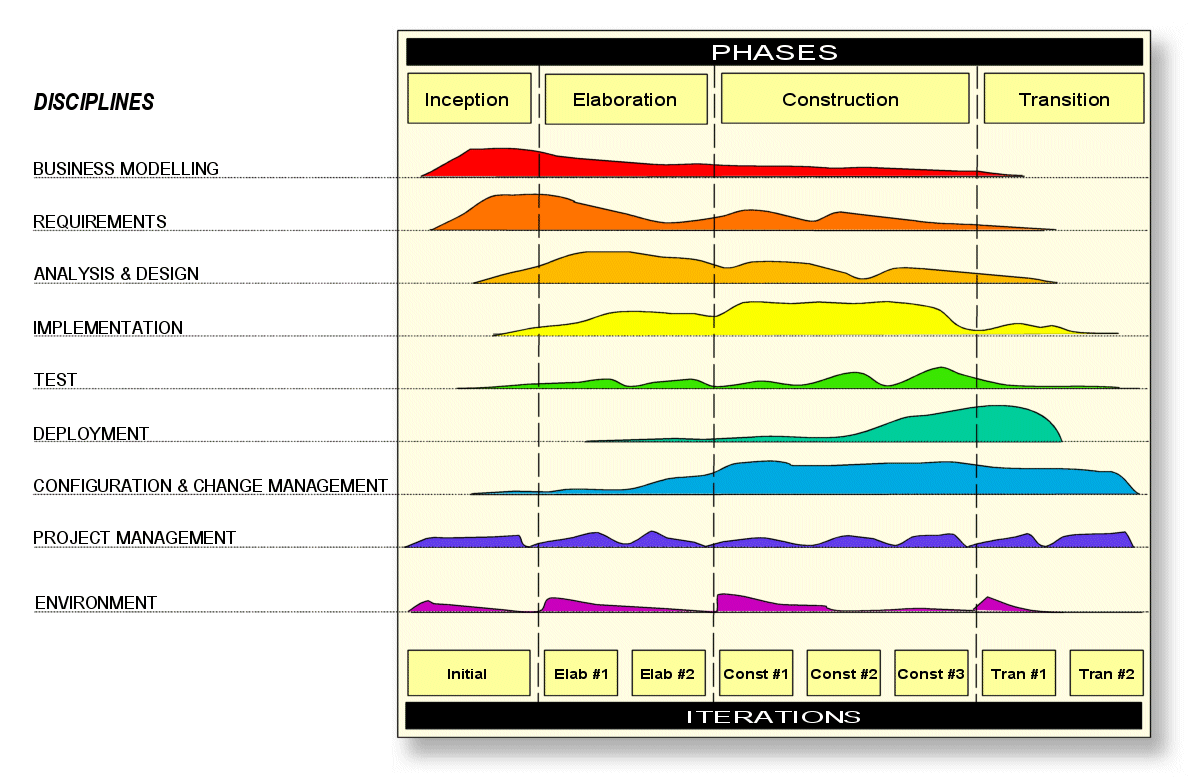
\includegraphics[width=0.80\textwidth]{Billeder/Udviklingsproces/RUP}
	\caption{RUP model}
	\label{fig:rup}
\end{figure}

\textbf{Inception}\\
Inception fasen er projektets indledende fase, og bruges til at lave forundersøgelse, valg af hardware/software samt opsætning af krav. I løbet af inception fasen udarbejdes foranalyse, indkøbsliste, krav til systemet og overordnet systemskitse. 

\textbf{Elaboration}\\
Elaboration fasen tager hånd om systemarkitektur og design. I denne fase udarbejdes der indledningsvis en domain model og derefter systemarkitektur af hardware og software. 

\textbf{Construction}\\
I construction fasen er produktet i fokus, og der skiftes løbende mellem implementering af ny funktionalitet, test og dokumentation af nytilføjet funktionalitet. 

\textbf{Transition}\\
Transition er den afsluttende fase, og tager hånd om færdiggørelse af projekt og overdragelse af produkt. Idet gruppen ikke har nogen egentlig kunde, bruges fasen til lave accepttest, færdiggøre dokumentation og udarbejdelse af rapport. 

\newpage

\subsubsection*{ASE modellen}
ASE modellen som ses på figur \ref{fig:dokument_udvikling} er brugt i kombination med RUP. RUP bruges til at danne overordnede rammer for projektet, mens ASE modellen bruges til definere hvilke dokumenter der skal udarbejdes og hvornår. På figur \ref{fig:dokument_udvikling} vise hvilke dokumenter der oprettes som produkt af ASE modellen. 

\begin{figure}[H]
	\centering
	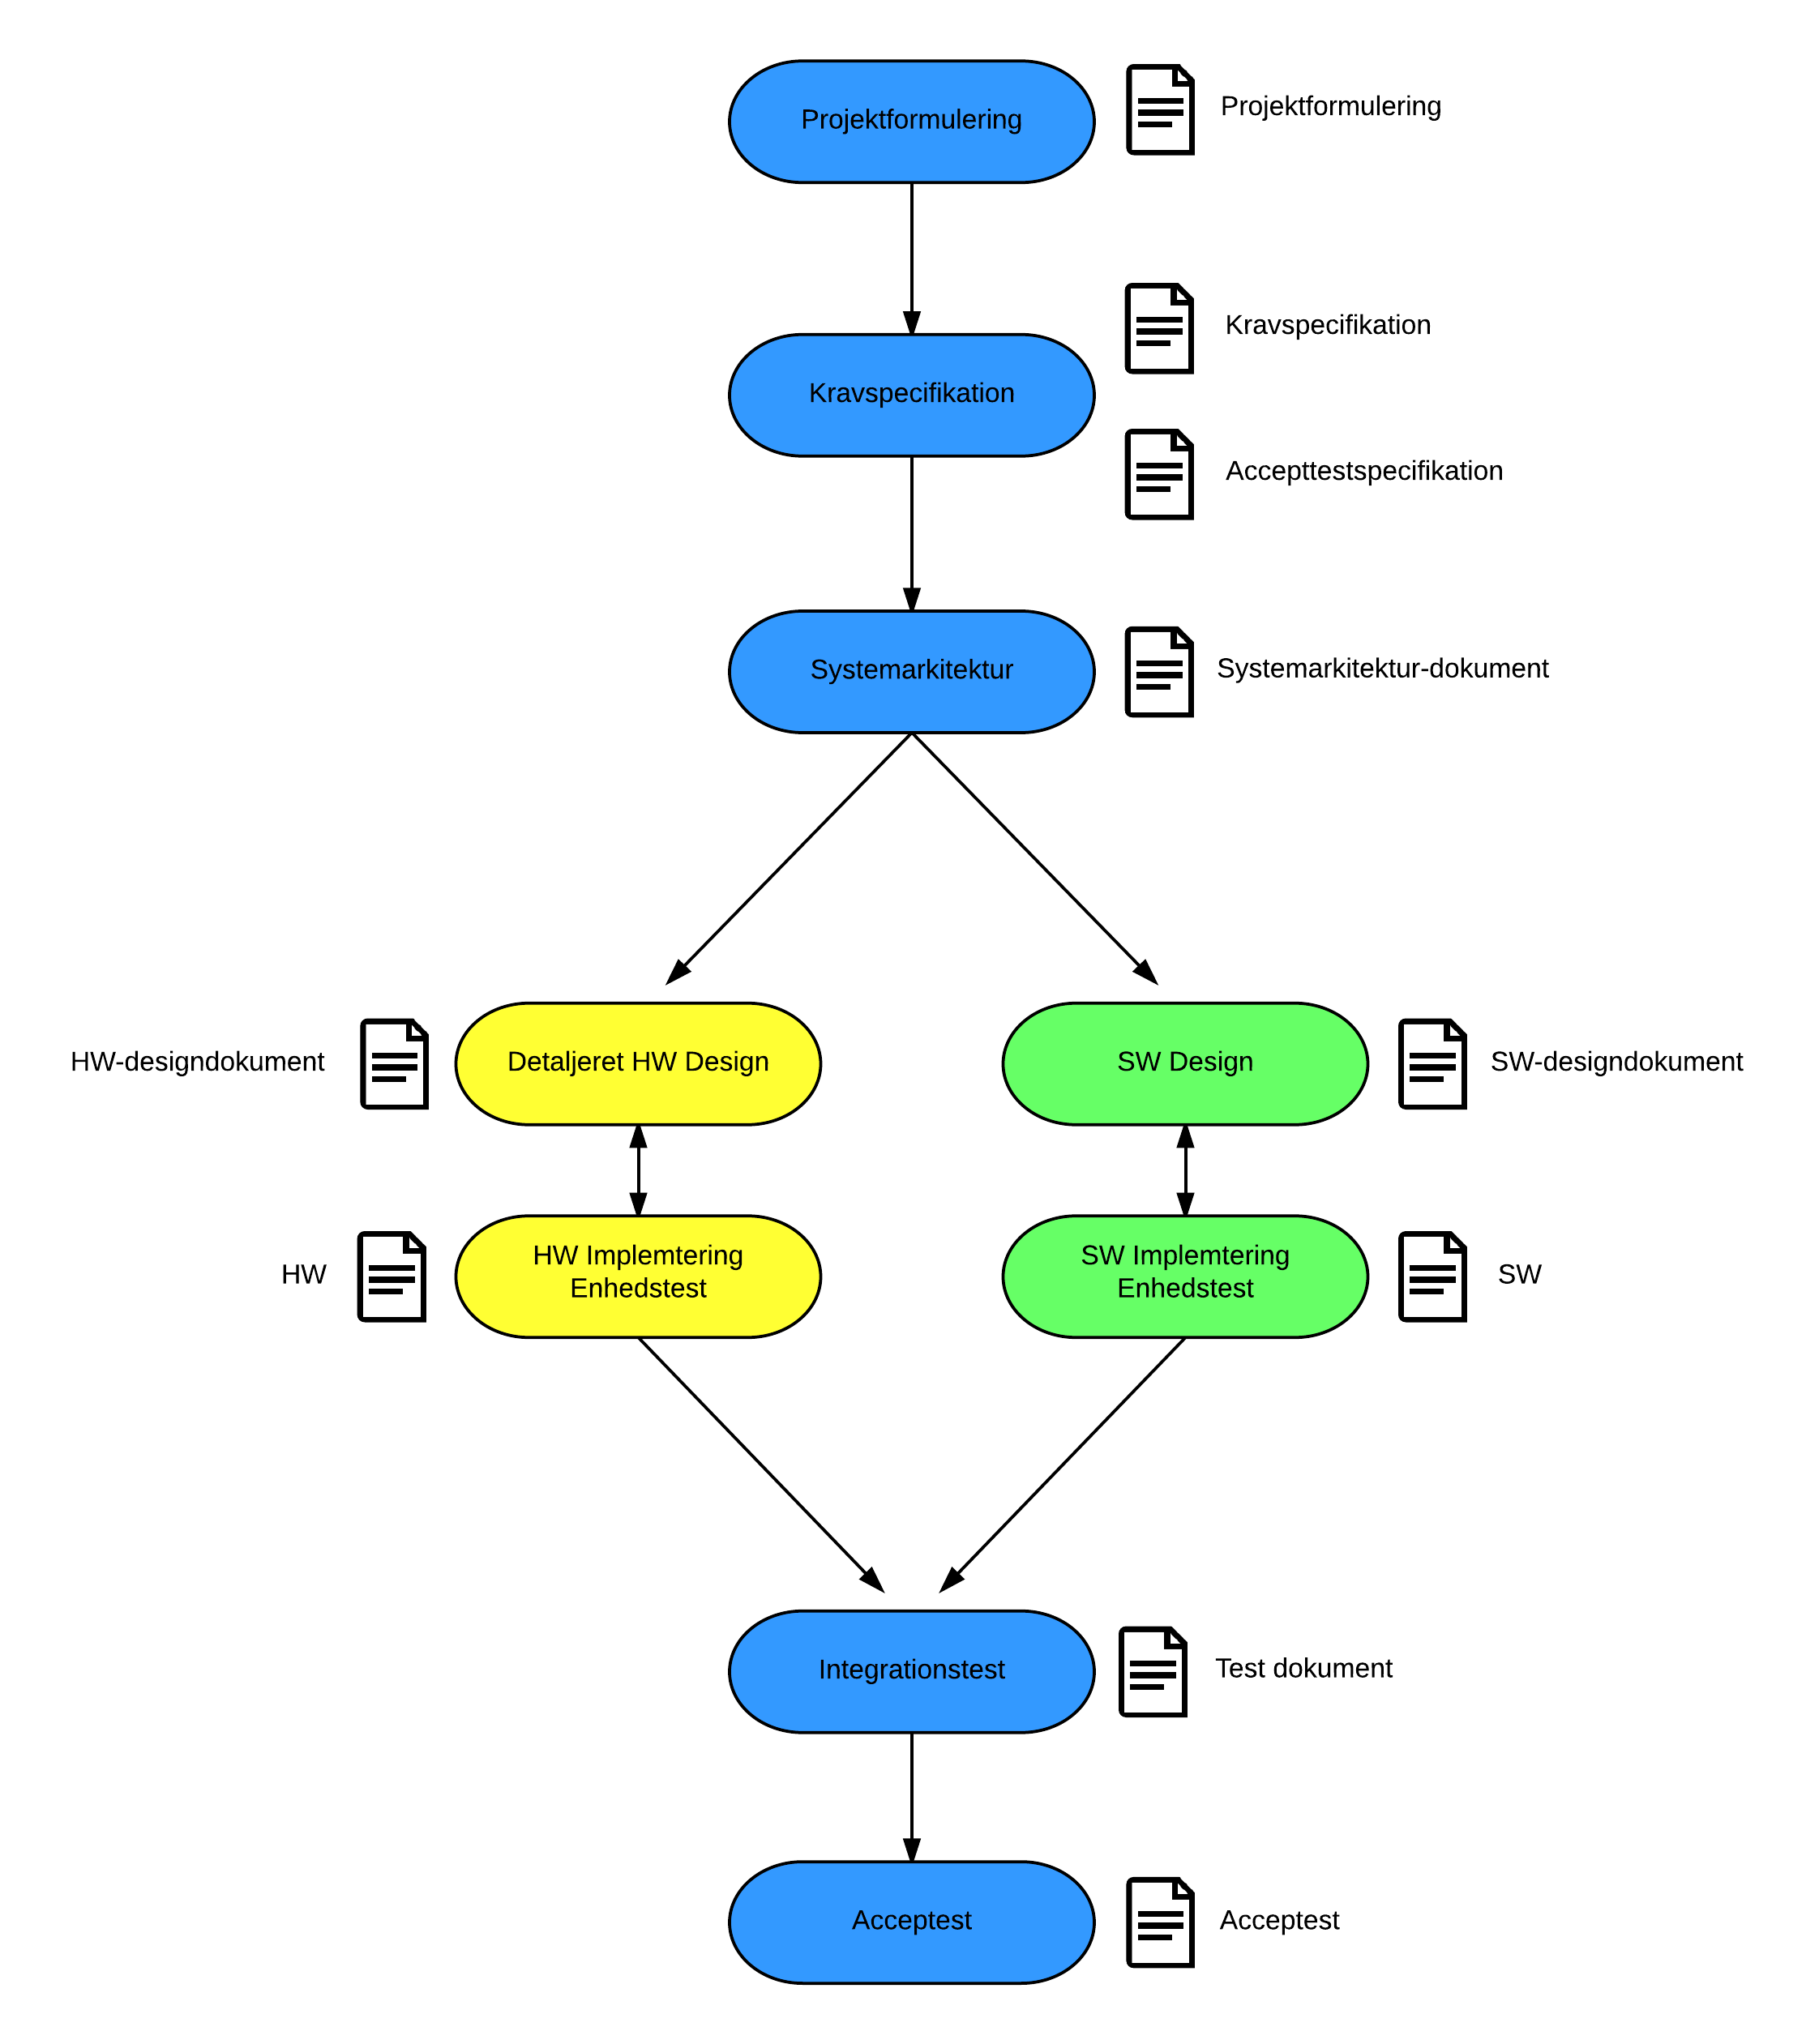
\includegraphics[width=1\textwidth]{Billeder/Udviklingsproces/ase_model}
	\caption{ASE modellen}
	\label{fig:dokument_udvikling}
\end{figure}

\newpage

\subsubsection*{N + 1 model}
Alt software design i projektet er lavet ud fra systemudviklings modellen N + 1 [X]. Modellen er en udviklingsmodel der beskriver software fra flere forskellige view's.  
Med N + 1 modellen tages der udgangspunkt i et use case view. Derefter er det op til udviklerholdet at bestemme hvor mange views der skal bruges for at beskrive systemet på tilstrækkelig vis. 

Til beskrivelse af systemets software anvendes en 5 + 1 view model, som indeholder use case view, logical view, process view, data view, deployment view og implementation view. 
På figur \ref{fig:n+1} ses en illustration der viser 5 + 1 modellen.
5 + 1 modellens view's beskrives uddybende på den følgende side. 

\begin{figure}[H]
	\centering
	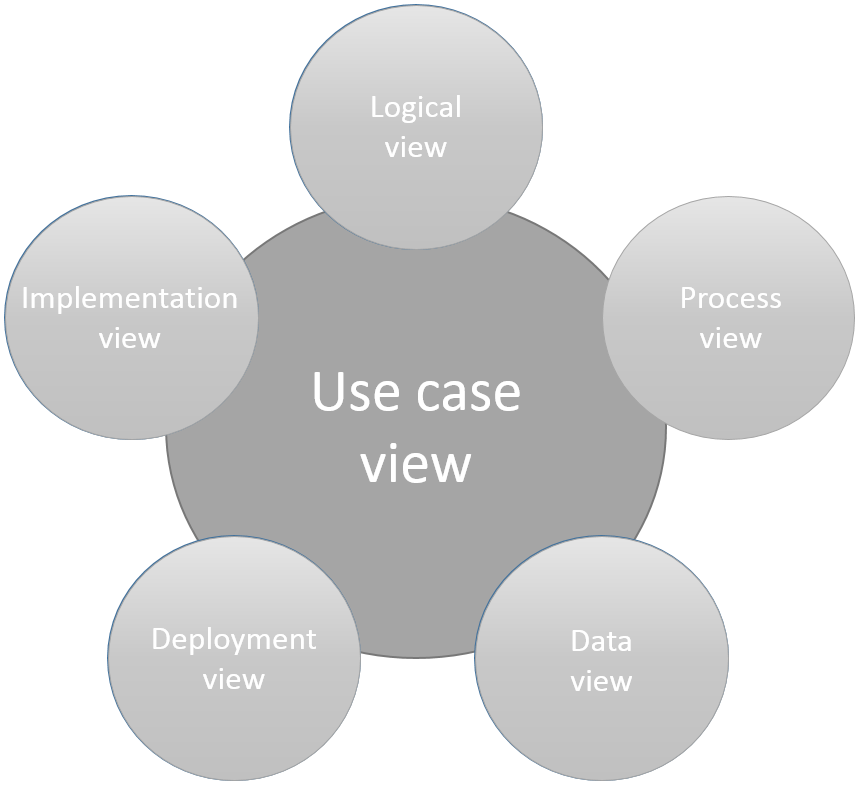
\includegraphics[width=0.7\textwidth]{Billeder/Udviklingsproces/n+1}
	\caption{5 + 1 model}
	\label{fig:n+1}
\end{figure}

\newpage


\textbf{Use case view}\\
Use case viewet består af use case beskrivelser, der er udviklet ud fra brugers synspunkt og som bruges til at beskrive systemets funktionalitet og forskellige brugsscenarier. Alle udarbejdede use case beskrivelser forefindes i kravspecifikationen.

\textbf{Logical View}\\
Logical view bruges til at beskrive de logiske blokke i systemet. På baggrund af hver iteration, er der udarbejdet tilhørende designoverview-, pakke-, klasse-, sekvens- og state machine diagrammer. Diagrammerne bruges til at give et overblik over systemets funktionalitet på et mere detaljeret niveau.

\textbf{Process View}\\
Process view bruges til at beskrive sideløbende processer/tråde i systemet og hvordan samspillet imellem disse er. I view'et beskrives også krav til timing i kommunikation mellem drone og server.

\textbf{Data View}\\
I data viewet beskrives layout af data der gemmes i systemet og hvordan det lagres. Desuden beskrives hvordan data sendes rundt i systemet og hvordan servers database tilgås.

\textbf{Deployment View}\\
Deployment view beskriver systemets grundlæggende fysiske elementer og sammenspillet mellem dem. I view'et beskrives også hvilke software pakker der bruges i systemet og hvor de bruges. Desuden beskrives hvilke protokoller der er anvendt, fx. layout af meddelelser med header/start/stop

\textbf{Implementation View}\\
Implementation view beskriver vigtige elementer i systemet som ikke er blevet beskrevet i andre views. Bla. beskrives hvilke værktøjer der er benyttet til projektet og hvordan disse værktøjer er sat op. Det beskrives også hvilke filer systemet er bygget af og hvordan disse filer skal linkes sammen.


\newpage
\subsection{Udviklingsværktøjer}
I dette afsnit beskrives de udviklingsværktøjer [X] der er benyttet i løbet af projektet. \\

\textbf{Latex}\\
Latex er benyttet til udarbejdelse af dokumentation og rapport. 

\textbf{Git}\\
Git er versionsstyring og fildelings værktøj.

\textbf{Lucidchart}\\
Lucidchart er benyttet til udarbejdelse af software diagrammer.

\textbf{Visio}\\
Visio er benyttet til udarbejdelse af hardware diagrammer.

\textbf{Atmel studio 6.2}\\
Atmel studio er det IDE hvor kode til main controller skrives.

\textbf{Arduino IDE}\\
Arduino IDE er brugt til at teste kode til main controller.

\textbf{Atom}\\
Atom er et IDE / tekstbehandlings program til håndtering kode.

\textbf{OSX ternimal}\\
Opsætning og programmering af server og webapplikation. 

\textbf{SQLite database}\\
SQLite er benyttet til systemets database.

%%%%%% Analyse %%%%%%
\chapter{Analyse}
\label{chap:analyse}

Efter at have udarbejdet kravspecifikation, var der formet en idé om hvordan systemet skulle fungere. 
I dette afsnit beskrives tanker og overvejelser der på baggrund af kravspecifikation er gjort i projektets indkøbsfase. 
Først beskrives det hvad systemet krævede af hardware og software komponenter. 
Dernæst beskrives hvilke komponenter der blev valgt, og til sidst beskrives begrundelse for gruppens valg. 

\newpage

Efter at have udarbejdet kravspecifikation og systemskitse, var der formet en idé om hvordan systemet skulle fungere. 
Nedenfor er der vist udkast til den funktionalitet drone, webapplikation, server og database var tiltænkt at have: \\

\textbf{Dronen skal kunne:}\\
Finde egen flyvehøjde\\
Finde egen orientering.\\
Finde egen GPS position.\\
Beregne korrekt flyveorientering. \\
Kommunikere med server via mobilt netværk.\\

\textbf{Webapplikation, server og database skal:}\\
Give bruger adgang til monitorering af tidlige flyvninger.\\
Benyttes af bruger til at lave nye flyveopsætninger.\\



I dette afsnit beskrives tanker og overvejelser der på baggrund af kravspecifikation er gjort i projektets indkøbsfase. 
Først beskrives det hvad systemet krævede af hardware og software komponenter. 
Dernæst beskrives hvilke løsninger der blev valgt, og til sidst beskrives begrundelse for gruppens valg. 



\newpage

\section{Drone}
Dronen var den mest essentielle del der skulle købes i indkøbsfasen. Derfor beskrives overvejelser lavet i forbindelse med drone indkøb som det første.

Da den rette dronen skulle finde blev der lagt vægt på: \\
\textit{Pris}    \\
\textit{Løftekapacitet}\\
\textit{Tilgængelighed af reservedele} \\
\textit{Open source kode til regulering} \\

Ud fra kriterierne stod valget mellem 3D Robotic's eller AeroQuad's quadrocopter.

\textbf{3D Robotic}\\
Ved køb af 3D Robotics quadrocopter fik man motor controller board, motorer der kunne yde op til 850 Kv, 10" propeller og 20 ampere electronic speed controllers. Foruden dette var styringssoftware open source.

\textbf{AeroQuad}\\
AeroQuad's ARF Cyclone quadrocopter var større, havde 12” propeller og motorer der kunne yde 950 Kv. Ligesom det var tilfældet med 3DR's quadrocopter medfulgte der styringssoftware samt controller board og 20 ampere electronic speed controller.\\  

Aeroquad’s quadrocopter blev valgt fordi den havde større vingefang og motorer med højere ratationshastighed, hvilket betød øget løfteevne og stabilitet. Desuden var Aeroquad’s quadrocopter en smule billigere end 3D robotic's. 





%%%% Kilder %%%%
\begingroup
\raggedright
\bibliography{bibtex/litteratur}							
% Litteraturlisten inkluderes
\endgroup

%%%% Fixme-listen %%%%
\newpage														% Ny side til Fixme-listen
%\listoffixmes													% Fixme-listen - fjernes til sidst i projektet med "%"

%%%% Appendiks %%%%
\appendix														% Appendiks/bilag start - giver chapter bogstaver i stedet for tal
\clearforchapter												% Sikrer at pagestylen aktiveres paa den rigtige side
\phantomsection													% Kunstigt afsnit, som hyperlinks kan 'holde fast i'
\pdfbookmark[0]{Appendiks}{appendiks}							% Tildeler en klikbar bookmark til den endelige PDF

\end{document}													% Slutter dokumentet - obligatorisk